\documentclass{article}
\usepackage[left=0.5in,top=0.5in,right=0.5in,bottom=0.5in]{geometry}
\usepackage[english]{babel}
\usepackage[utf8]{inputenc}
\usepackage[table]{xcolor}
\usepackage{amssymb,amsmath,amsthm}
\usepackage{changepage,threeparttable}
\usepackage{booktabs,multirow}
\usepackage{graphicx}
\usepackage{soul}
\graphicspath{{./images/}}
\def\R#1{\(R_{\text{\tiny#1}}\)}
\def\V#1{\(V_{\text{\tiny#1}}\)}
\def\I#1{\(I_{\text{\tiny#1}}\)}
\def\Rr#1{R_{\text{\tiny#1}}}
\def\Vv#1{V_{\text{\tiny#1}}}
\def\RDIV{\(\frac{R_{\text{1}}}{R_{\text{1}}+R_{\text{2}}}\)}
\def\VDIV{\(\frac{V_{\text{1}}}{V_{\text{12}}}\)}
\title{Lab 5: Voltage Divider}
\author{Philip Kim}
\date{\today}
\begin{document}
\maketitle
\vspace*{-1cm}
\begin{table}[!htp]\centering
  \subsection*{Part 1}
  \begin{tabular}{|c|c|c|c|c|c|c|c|}\hline
  \multicolumn{7}{|c|}{\textbf{Table 1: Series Resistors}} \\\hline
  \R{1} & \R{2} & \V{1} & V/DIV for \V{1} & \V{12} & \RDIV\ & \VDIV\ \\\hline
  1k & 2k & 0.68V & 1V & 2.02V & 0.33k & 0.34V \\\hline
  1k & 100 & 1.85V & 1V & 2.02V & 0.91k & 0.92V \\\hline
  1k & 4.7k & 0.33V & 1V & 2.02V & 0.18k & 0.16V \\\hline
  1k & 10k & 0.16V & 1V & 2.02V & 0.09k & 0.08V \\\hline
  1k & 100k & 0.019V & 10mV & 2.02V & 0.0099k & 0.0094    V \\\hline
  \end{tabular}
  \begin{center}
    \subsection*{Picture 1}
    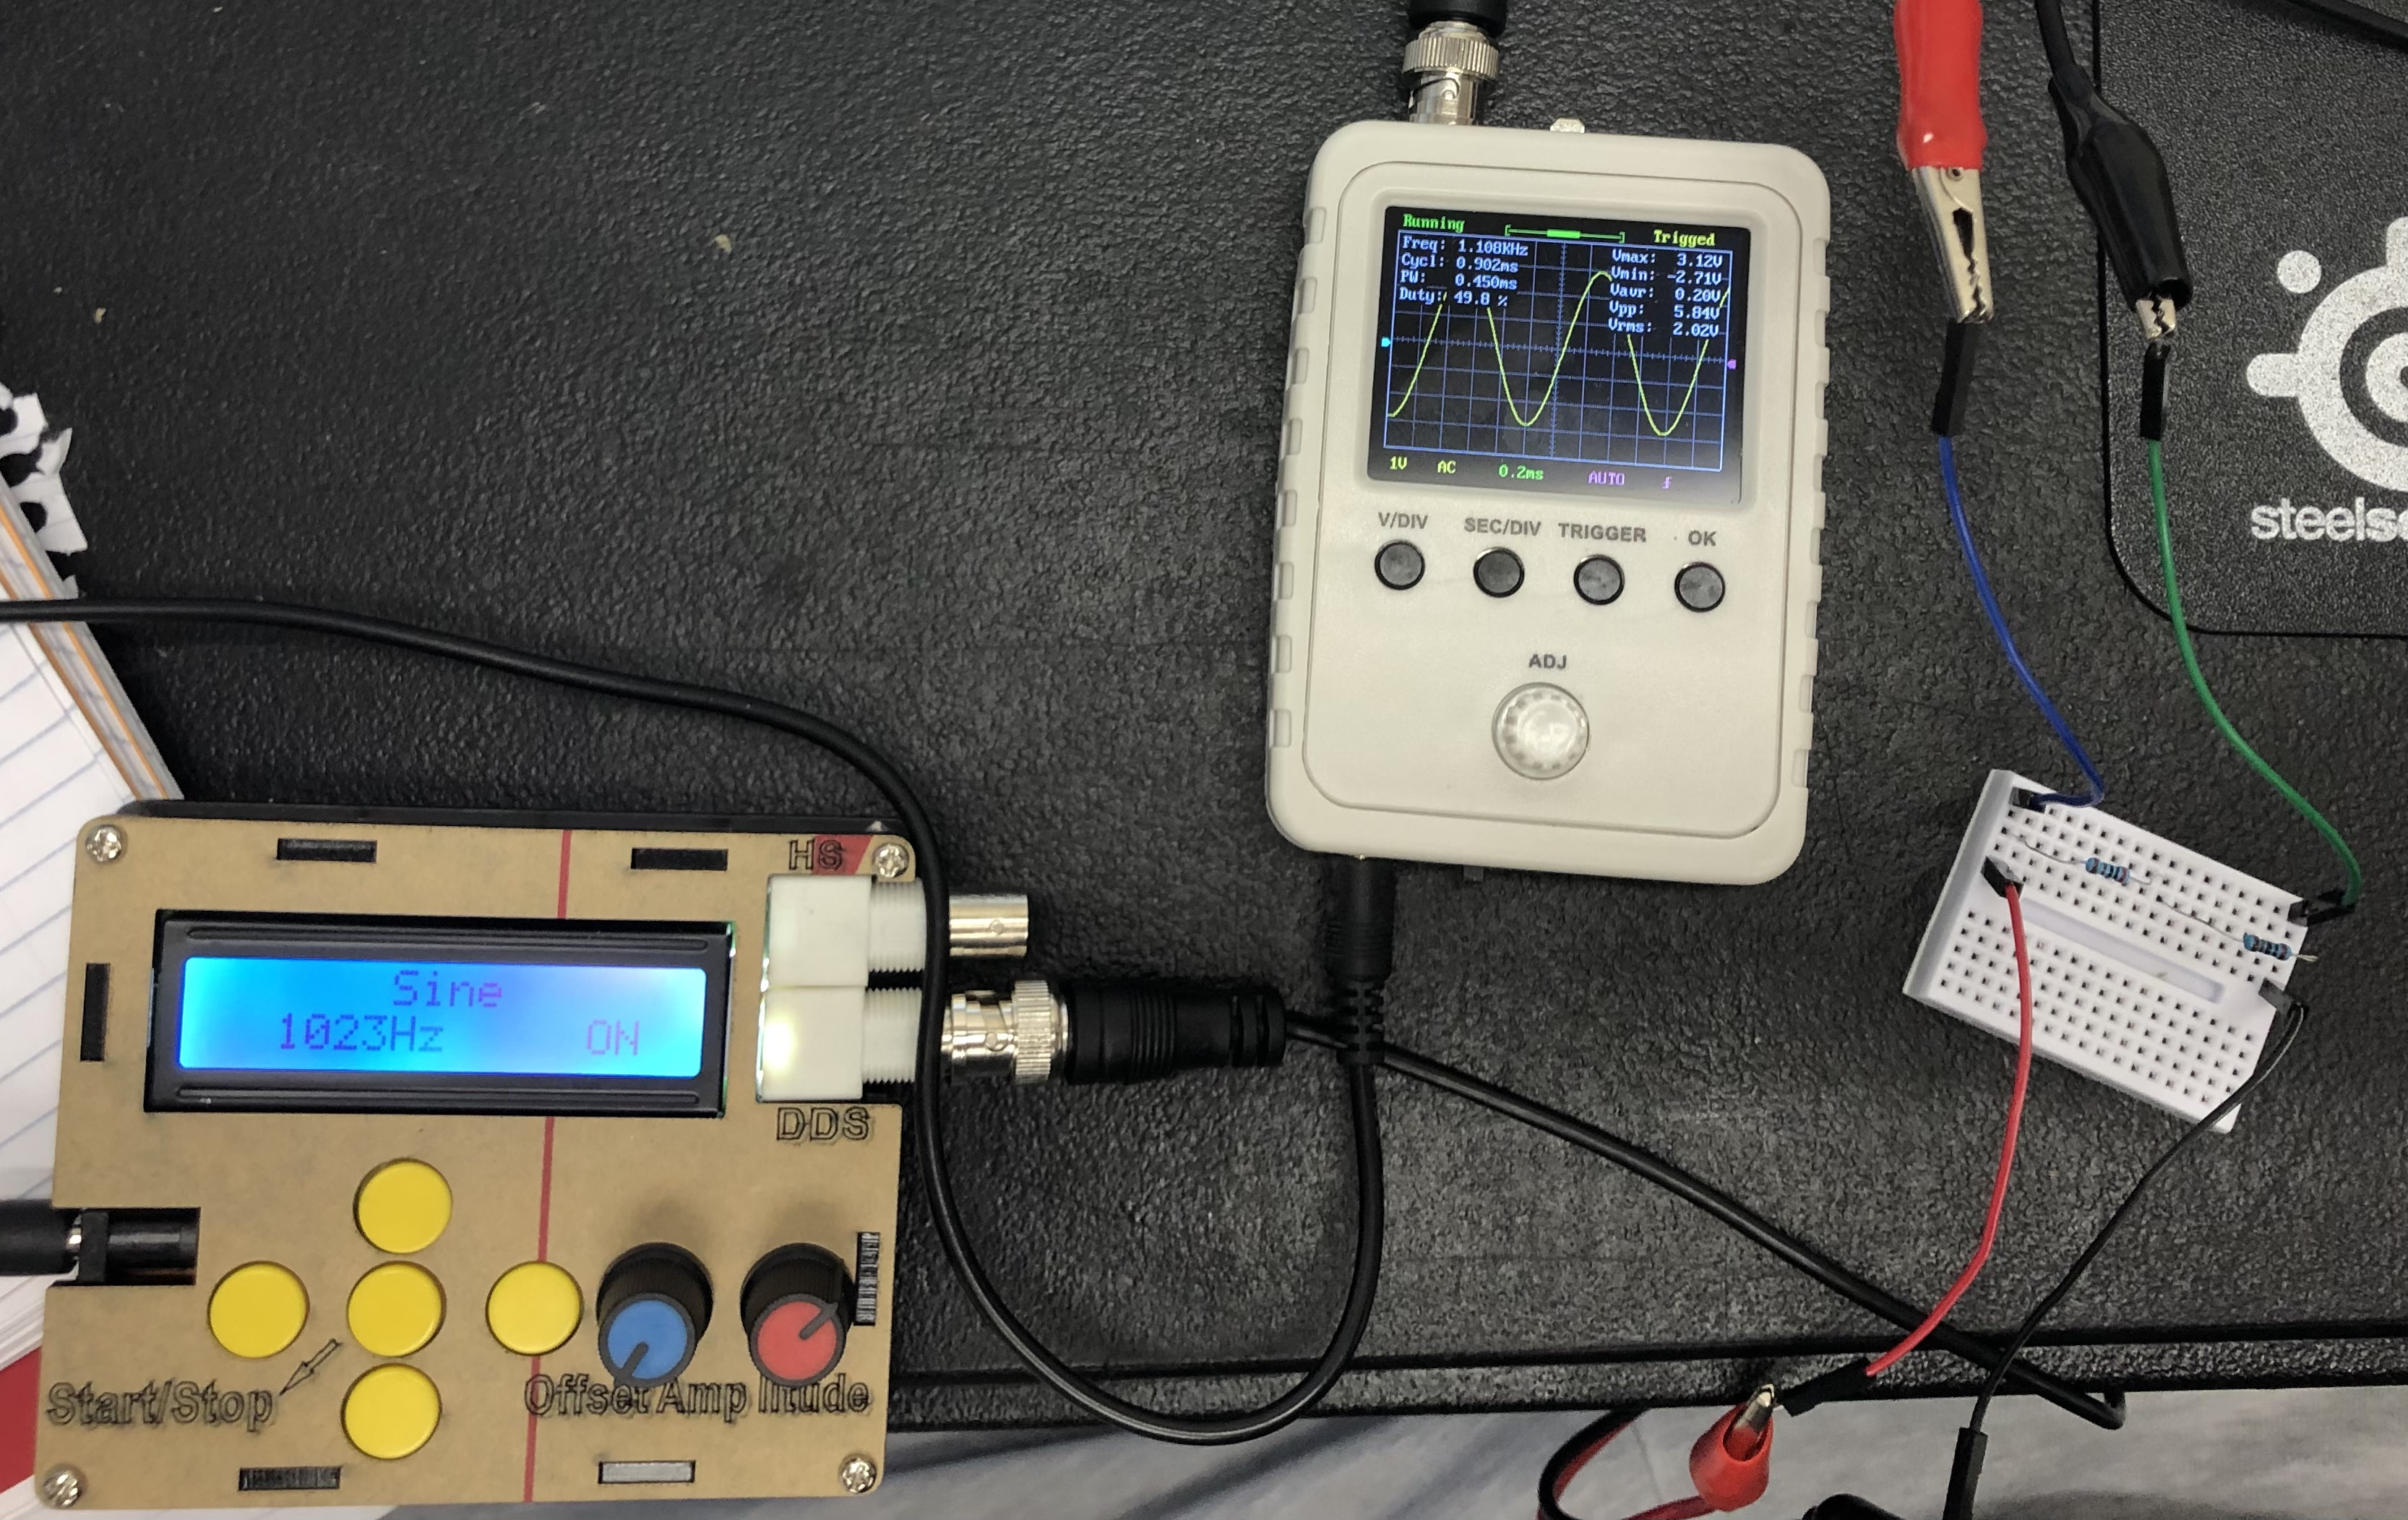
\includegraphics[width=8cm,height=4.5cm]{SV12.jpeg}
    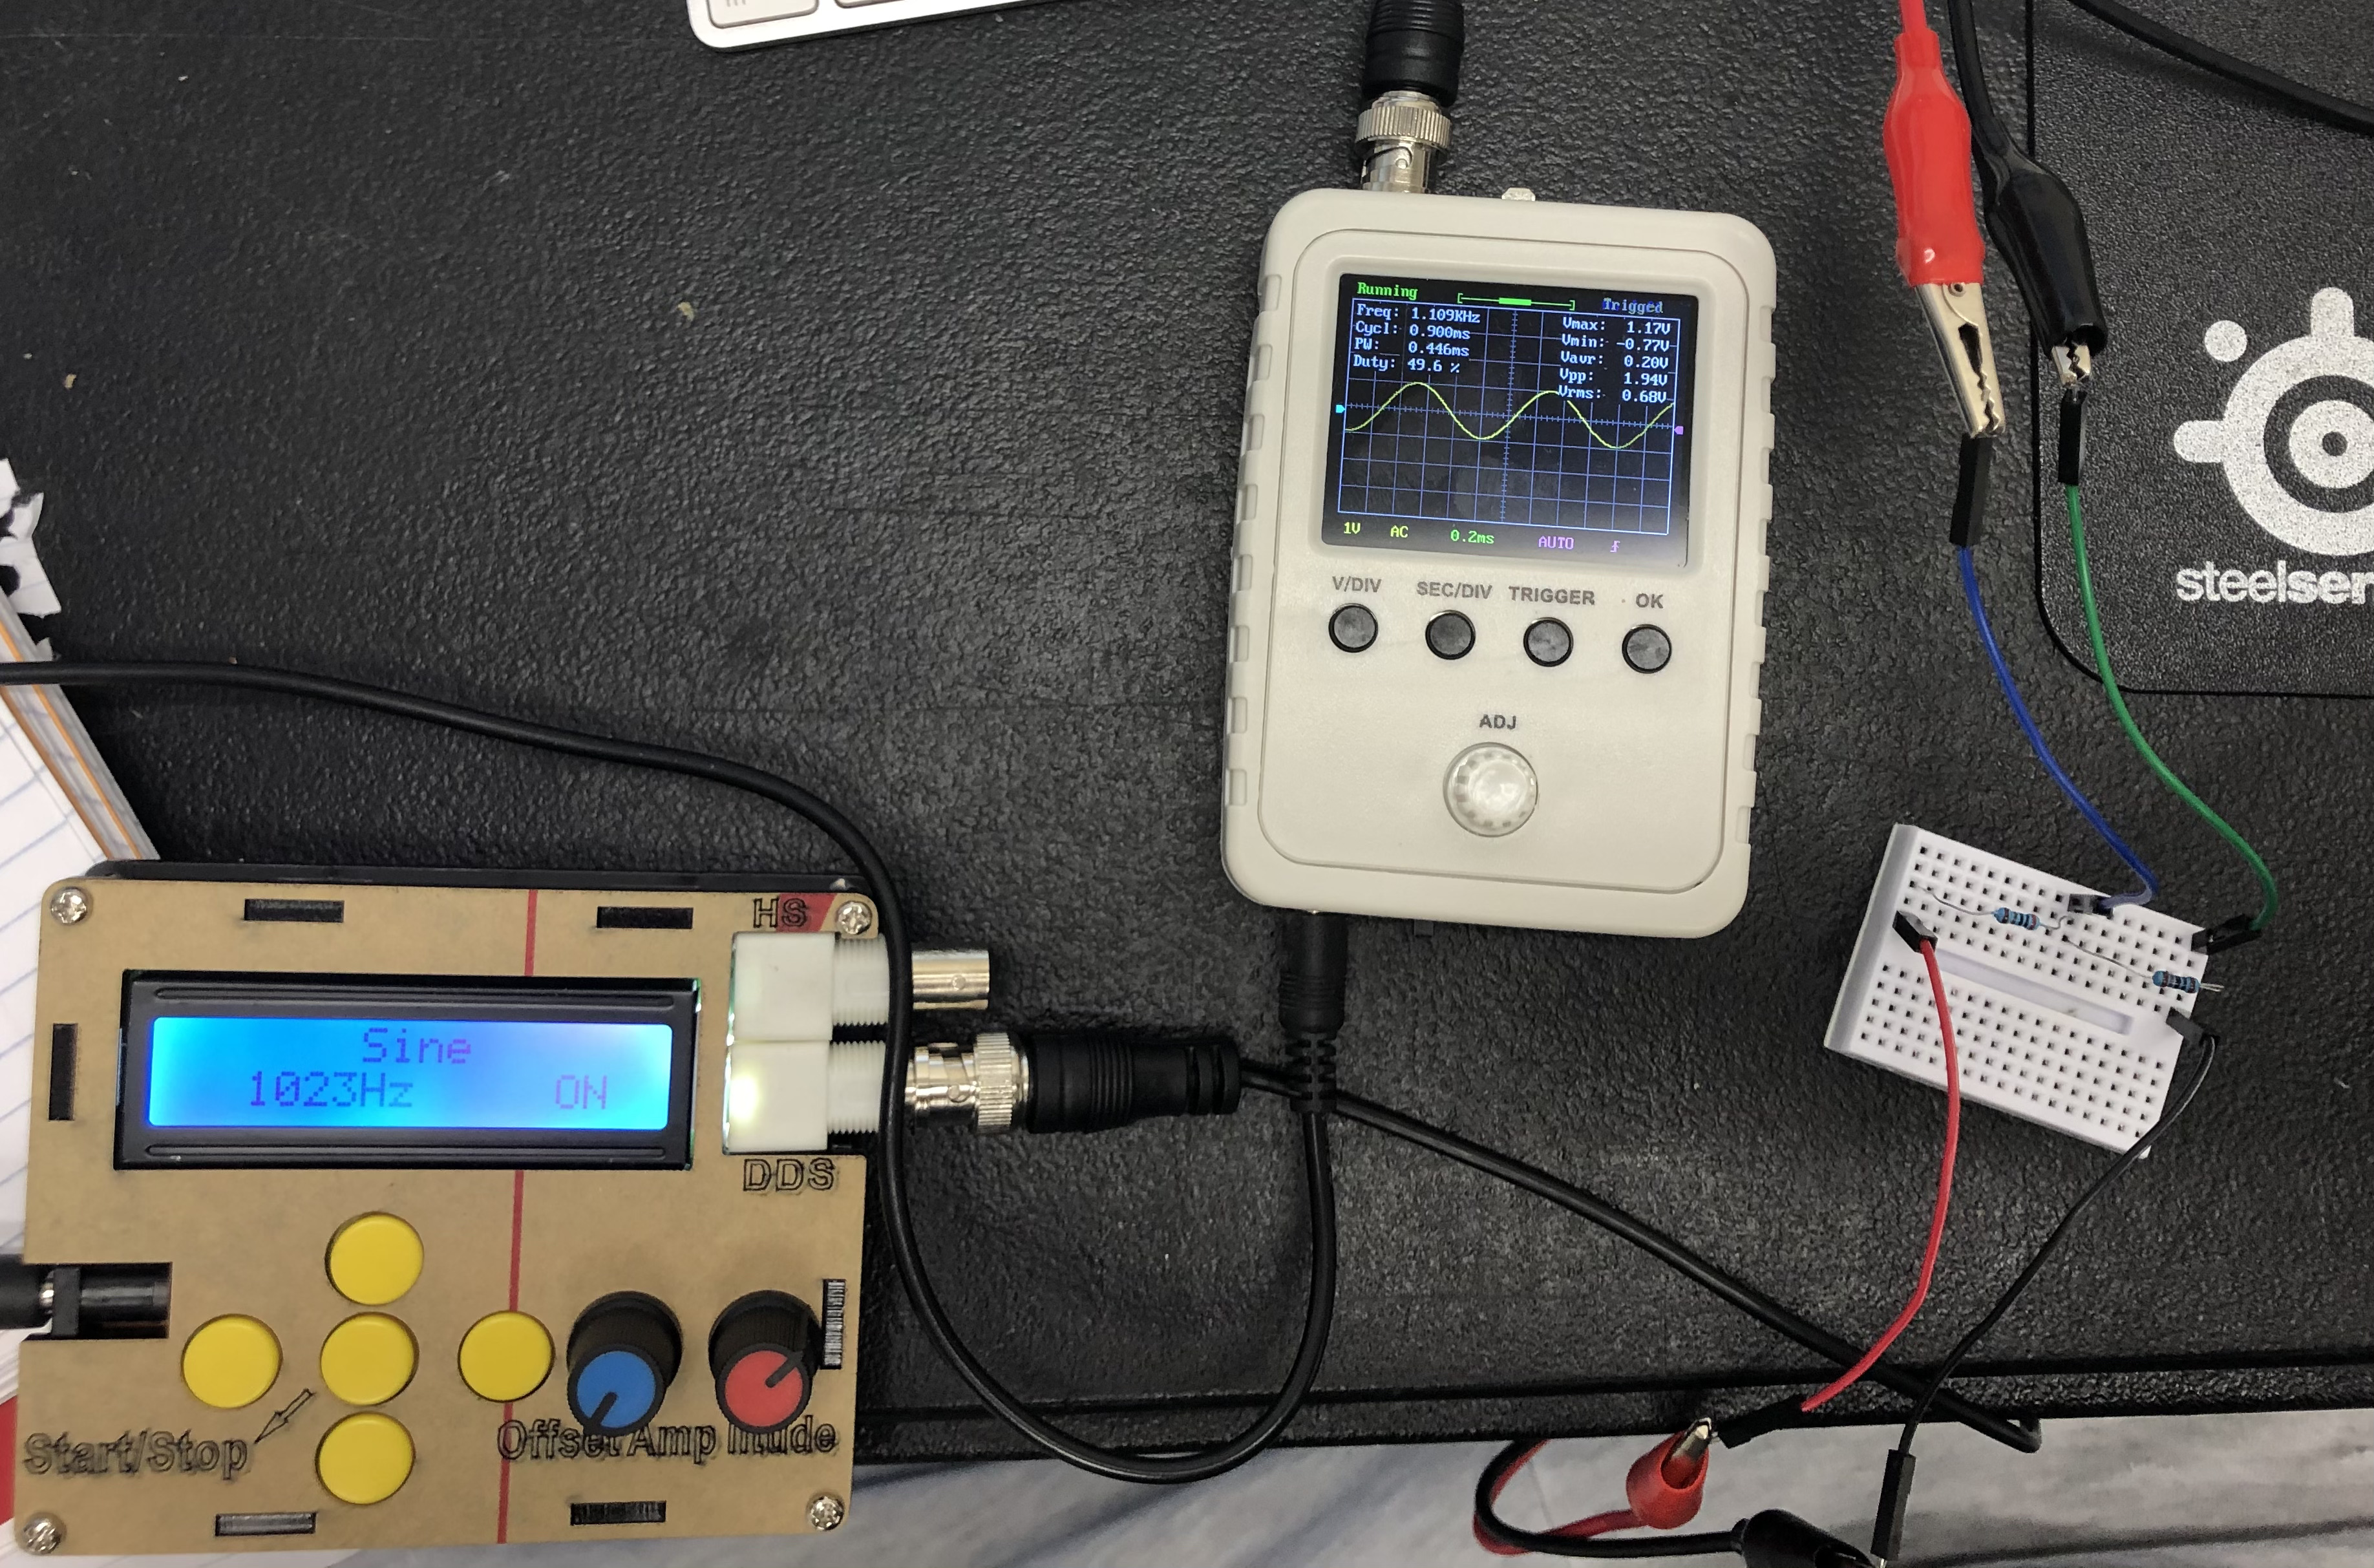
\includegraphics[width=8cm,height=4.5cm]{SV1.jpeg}
    \subsection*{Graph 1}
    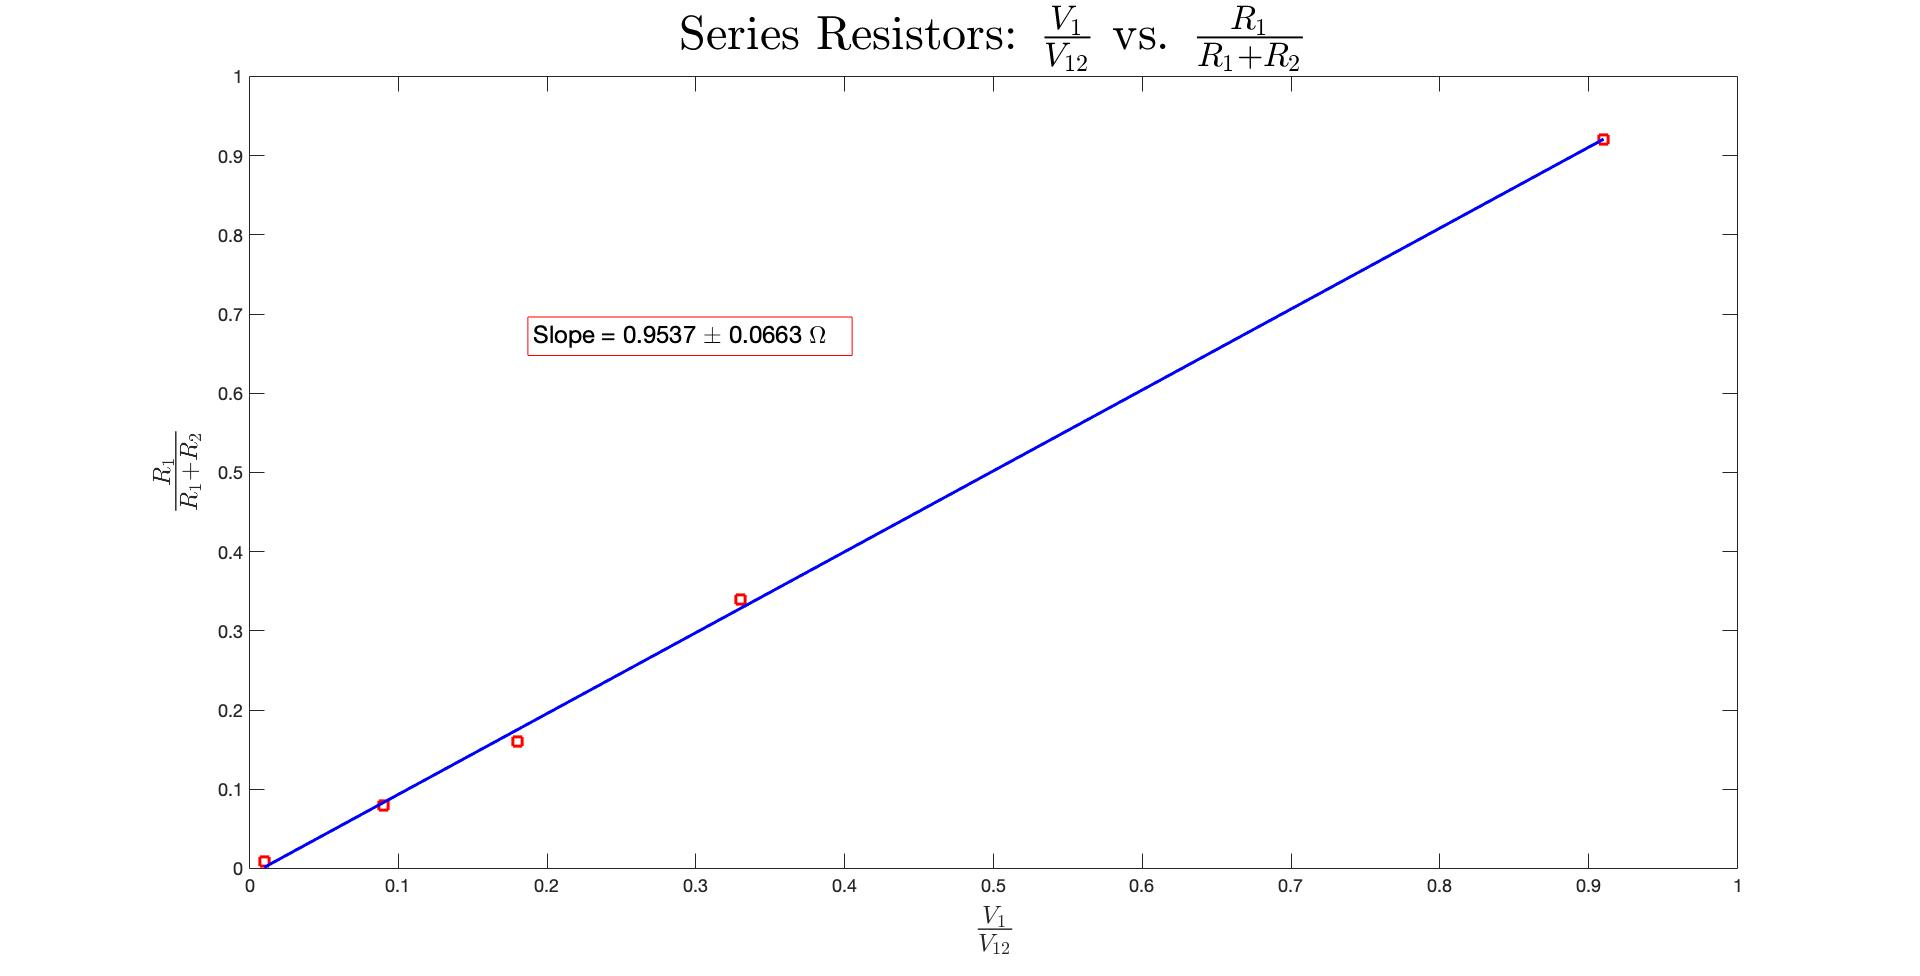
\includegraphics[scale=0.2]{series.jpg}
    \subsection*{Discussion 1}
    \begin{enumerate}
      \item What did you expect to see, and did you see it? If not, why not. If so, how well (quantitatively) did it fit your expectation?
      \begin{itemize}
        \item The \RDIV\ and \VDIV\ values are relatively the same with less than 10\% difference proving that the voltage divider is directly proportional to the input voltage and the ratio of \(R_1\) and \(R_{2}\).
      \end{itemize}
    \end{enumerate}
  \end{center}
\end{table}
\newpage
\begin{table}[!htp]\centering
  \subsection*{Part 2}
  \begin{tabular}{|c|c|c|c|c|c|c|c|c|c|c|}\hline
  \multicolumn{10}{|c|}{\textbf{Table 2: Parallel Resistors}} \\\hline
  \R{1} & \R{2} & \R{3} & \V{1} & V/DIV for \V{1} &  \I{1} = \I{23} & \V{123} & \V{23} & \R{23,expt} & \R{23,theory} \\\hline
  1k & 2k & 2.2k & 0.97V & 1V & 0.97 & 2.02V & 1.05V & 1.08k & 1.05k \\\hline
  1k & 2k & 100 & 1.85V & 1V & 1.85 & 2.02V & 0.12V & 91.9k & 95.24\(\Omega \) \\\hline
  1k & 2k & 4.7k & 0.85V & 1V & 0.85V & 2.02V & 1.17V & 1.38k & 1.40k \\\hline
  1k & 2k & 10k & 0.77V & 1V & 0.77 & 2.02V & 1.25V & 1.62k & 1.67k \\\hline
  1k & 2k & 100k & 0.68V & 1V & 0.68V & 2.02V & 1.34V & 1.97k & 1.96k \\\hline
  \end{tabular}
  \begin{center}
    \subsection*{Picture 2}
    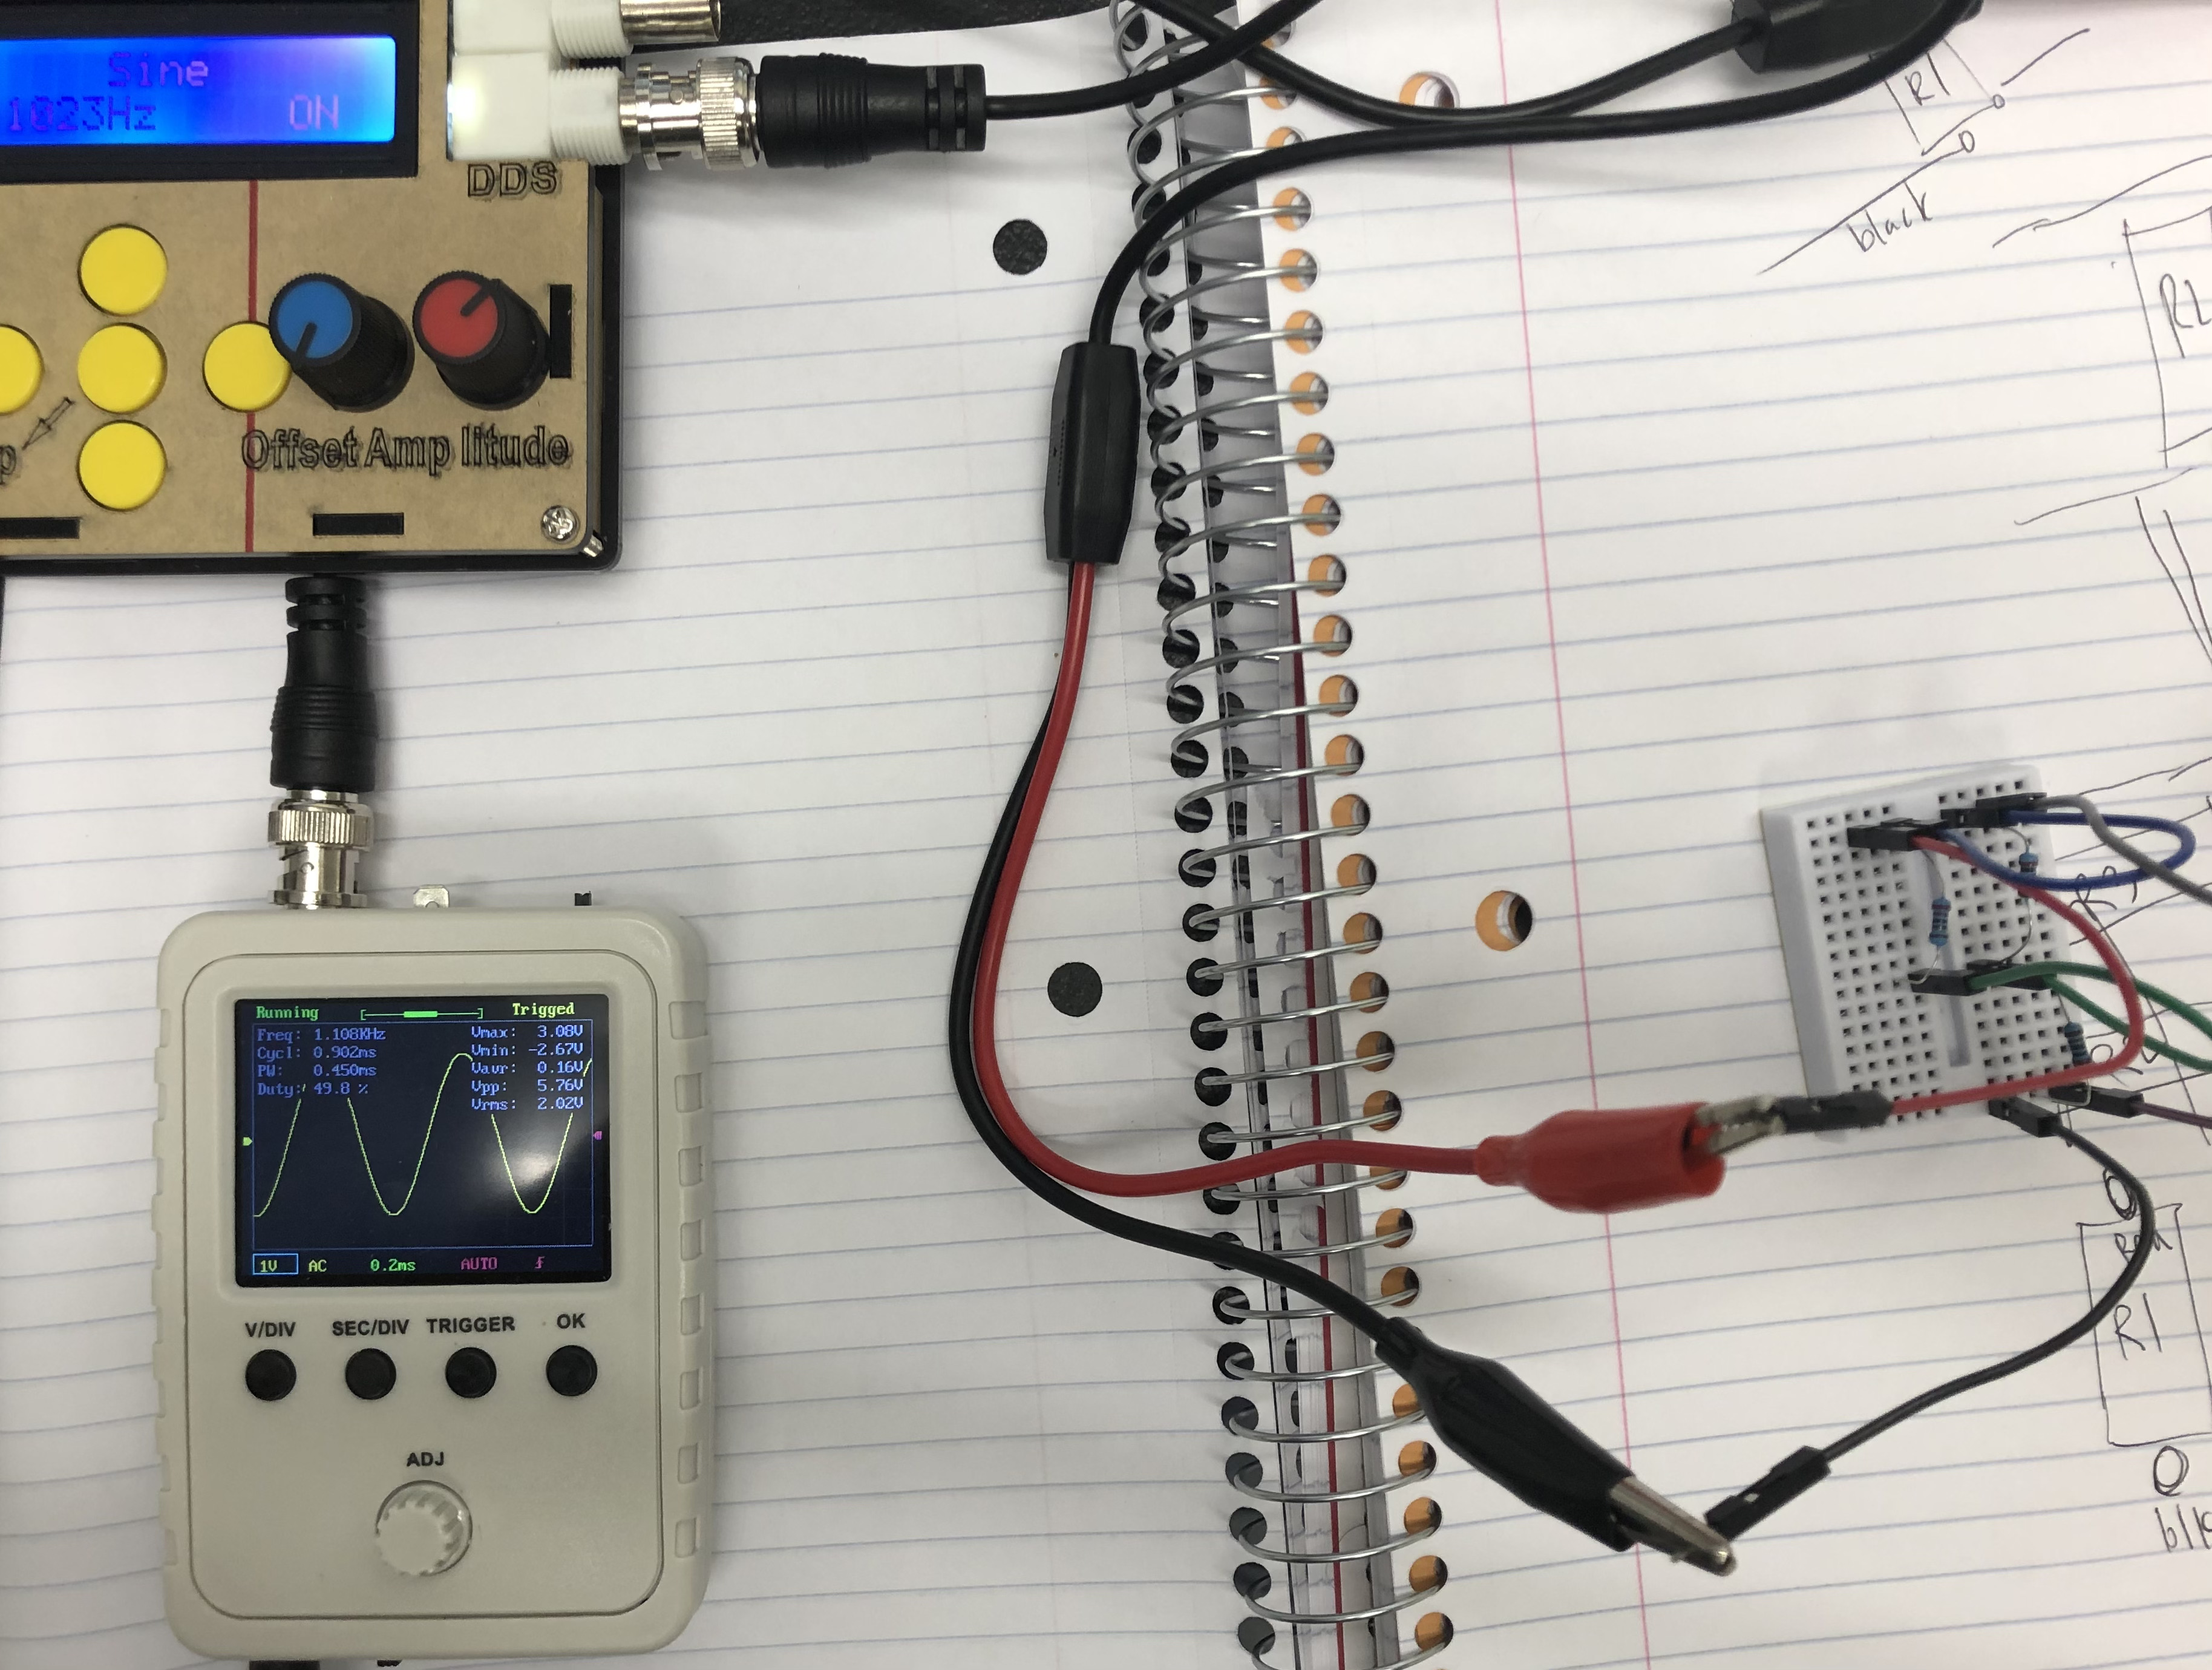
\includegraphics[width=8cm,height=6cm]{V123.jpeg}
    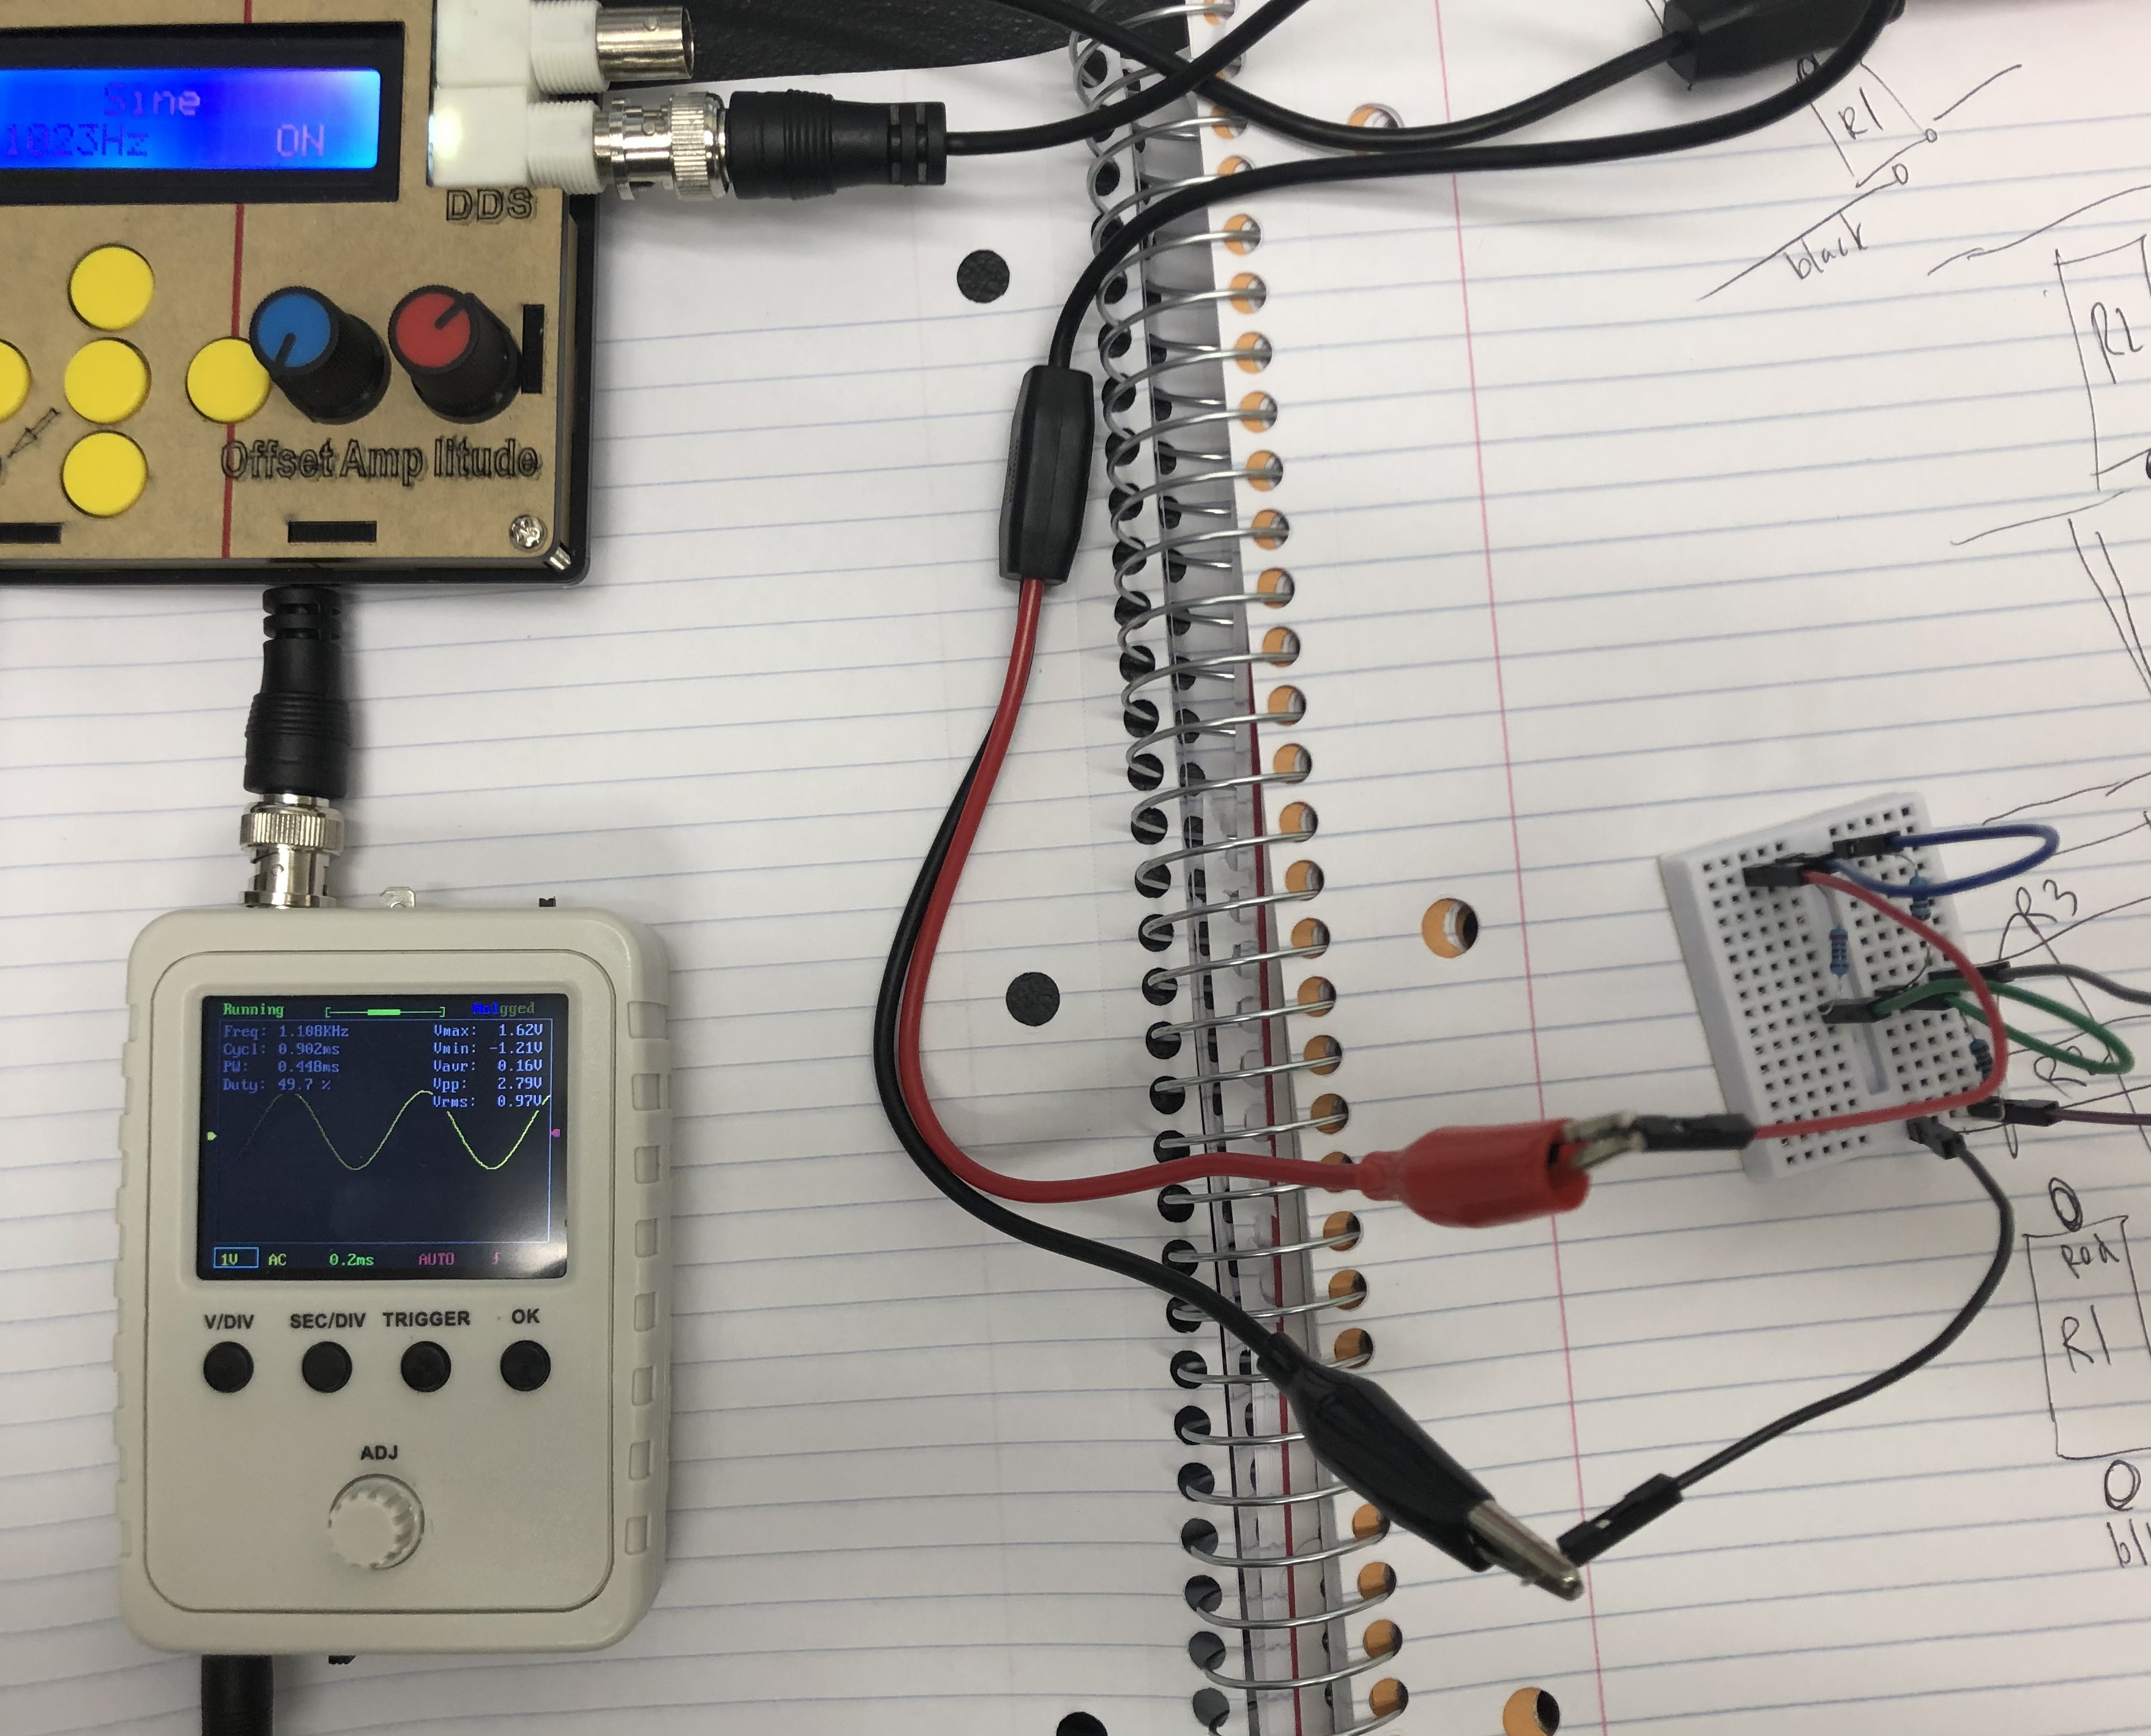
\includegraphics[width=8cm,height=6cm]{VP1.jpeg}
    \subsection*{Graph 2}
    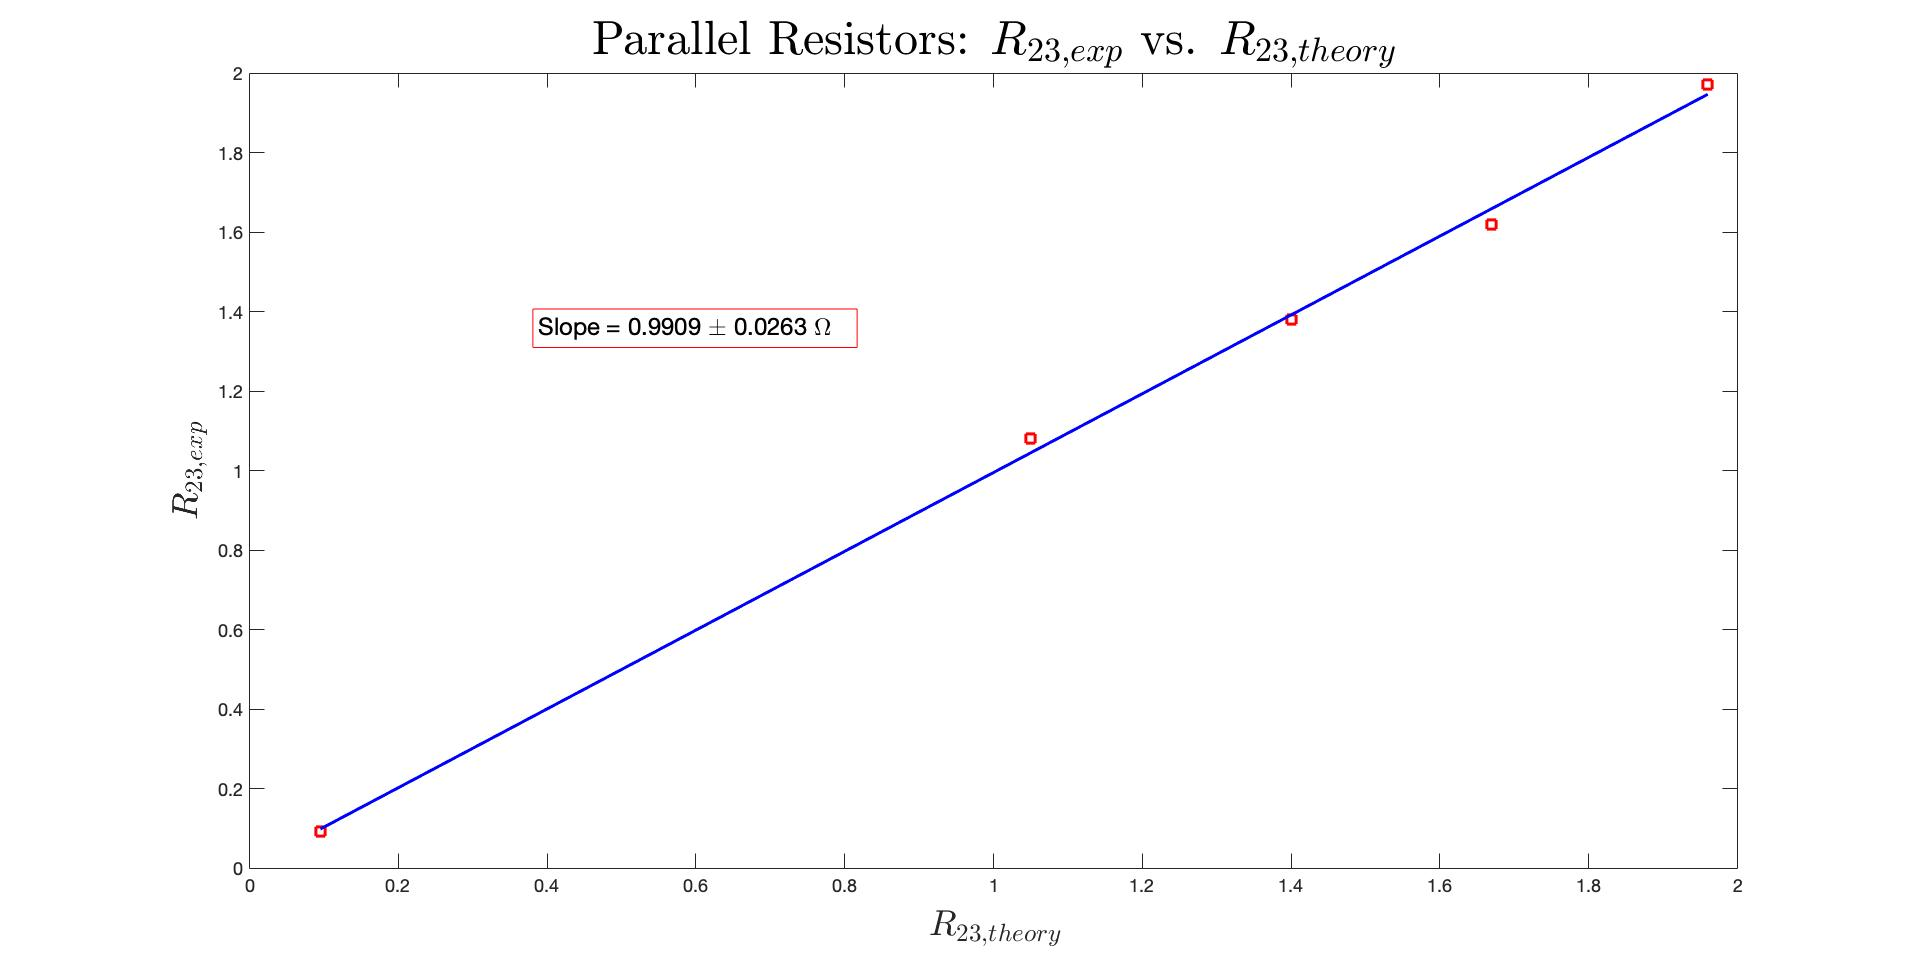
\includegraphics[scale=0.2]{parallel.jpg}
    \subsection*{Discussion 2}
    \begin{enumerate}
      \item What did you expect to see, and did you see it? If not, why not. If so, how well (quantitatively) did it fit your expectation?
      \begin{itemize}
        \item The experimental and theoretical values are relatively the same with less than 10\% difference proving that the voltage divider is directly proportional to the input voltage and the ratio of \(R_1\) and \(R_{23}\).
      \end{itemize}
    \end{enumerate}
  \end{center}
\end{table}
\end{document}
